\documentclass[../Main/main.tex]{subfiles}
\begin{document}
	\chapter{Finite volume method}
	\graphicspath{{../Finite volume method/figs/}}
	Finite volume methods are designed such that the conservation law we solve hold everywhere in the domain. Consider our elliptic model problem \eqref{eq:poisson}, first we divide our domain $\Omega$ into convex quadrilaterals(control volumes, cells), $\left \{ \Omega_i \right \}_i$. Then we integrate our equation over $\Omega_i$ and use the divergence theorem:
\begin{equation}\label{eq:fvm1}
	\int_{\Omega_i} -\nabla \cdot \pmb{K} \nabla u dx = -\int_{\partial \Omega_i} \pmb{K}\nabla u \cdot \pmb{\hat{n}} ds = \int_{\Omega_i} F dx
\end{equation}
The above equation equates the fluxes trough the boundary of a control volume with the source or sinks inside the control volume, the finite volume methods are discrete versions of this. The main idea is to approximate the normal flux trough edge $j$ of $\partial \Omega_i$
\begin{equation}
	f_{i,j} =-\int_{\partial \Omega_{i,j}} \pmb{K}\nabla u \cdot \pmb{\hat{n}} ds
\end{equation}

by a linear combination of $u_i$ at neghbouring cell centers. 
\begin{equation}
	\tilde{f}_{i,j} = \sum_{k}t_{j,k}u_k
\end{equation}
Where the \emph{transmissibility } $t_{j,k}$ has the property $\sum_k t_{j,k} = 0$. 
We also approximate the integral on the right side by evaluating $F$ at the cell center and multiply by the area of $\Omega_i$. We then end up with a system of equations
\begin{equation}\label{eq:fvm system}
	\sum_{j=1}^4 \tilde{f}_{i,j} = |\Omega_i|F(x_i)
\end{equation}
The system of equations \eqref{eq:fvm system} ensures local mass conservation. We will discuss different ways of constructing the transmissibility coefficients, as they result in very different discretizations.
\section*{Two point flux approximation}
\addcontentsline{toc}{section}{Two point flux approximation}The simplest way of constructing $t_{j,k}$ is also the most popular in the industry. As the name suggests, we only use the function value at two points, $x_{j,0}$ and $x_{j,1}$, to compute the numerical flux $\tilde{f}_j$.
\begin{figure}[H]
	\centering
	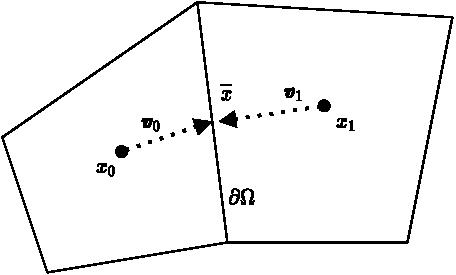
\includegraphics[width=0.5\textwidth]{two point.pdf}
	\caption{The two point flux approximation(TPFA) setup.}
\end{figure}
Let $\pmb{v}_1$ be the vector from cell center $x_0$ to the midpoint of the edge between the cells, $\overline{x}$. Then we approximate the flux between the cells by

\begin{equation}
	f_0=-\int_{\partial \Omega} \hat{\pmb{n}}^T \pmb{K}_0  \frac{\pmb{v}_0}{\left \| \pmb{v}_0 \right \|} (u(\overline{x})-u(x_0))ds
\end{equation}

Or as

\begin{equation}
	f_1 = -\int_{\partial \Omega} \hat{\pmb{n}}^T \pmb{K}_1  \frac{\pmb{v}_1}{\left \| \pmb{v}_1 \right \|} (u(x_1)-u(\overline{x}))ds
\end{equation}	

Where $\hat{n}$ is the normal vector to edge between the cells.
Because we require flux continuity we have that 
\begin{equation}
	f_0 = f_1 = t_0 u_0 + t_1 u_1
\end{equation}
Where, as before, $t_0 + t_1 = 0 \Rightarrow t_0 = -t_1$. We now have three equations and three unknowns, $u(\overline{x})$, $t_0$ and $t_1$. To simplify, we introduce the quantity $T_i = \int_{\partial \Omega} \hat{\pmb{n}}^T \pmb{K}_i  \frac{\pmb{v}_i}{\left \| \pmb{v}_i \right \|} $ to represent the cell transissibility. So first we solve for $u(\overline{x})$:
\begin{equation}
	T_0(u(\overline{x})-u(x_0)) = T_1(u(x_1)-u(\overline{x})) \Rightarrow u(\overline{x}) = \frac{T_0 u_0 + T_1 u_1}{T_0 + T_1}
\end{equation}
Next we insert this into the expression for $f_0$ 
\begin{equation}
	f_0 = -T_0(u_(\overline{x})-u(x_0)) = t_0(u_0 - u_1) \Rightarrow t_0 = \frac{1}{\frac{1}{T_0}+\frac{1}{T_1}}
\end{equation}
Hence, the transmissibility is the harmonic mean of the local transmissibilities. This discretization has the \textbf{advantages}
\begin{itemize}
	\item The matrix in \eqref{eq:fvm system} is symmetric, this makes the resulting system easier to solve.
	\item A small stencil, ie. the matrix in \eqref{eq:fvm system} has a bandwith of five for two dimensional quadrilateral grids.
	\item The assembly of the matrix in \eqref{eq:fvm system} is fast, as you have an explicit expression for the transmissibilities.
	\item It is easy to implement
\end{itemize}
But there is no such thing as a discretization that has everything, and TPFA has one big \textbf{disadvantage}
\begin{itemize}
	\item It is not convergent when the grid is not alligned with the principal directions of $\pmb{K}$, also called $\pmb{K}$-orthogonality. This is demonstrated in the next chapter, see \ref{fig:mesh_trapezoidal_potentia}
\end{itemize}
\section*{O-method}
\addcontentsline{toc}{section}{O-method}
The O-method is a multi-point flux approximation method, these types of methods where developed to make control volume methods converge for grids that are not $\pmb{K}$-orthogonal. It is described in detail in  \cite{Aavatsmark2002}, I only give a brief introduction.
\\
Consider the control volumes in \ref{fig:dualmesh}.
\begin{figure}[H]
	\centering
	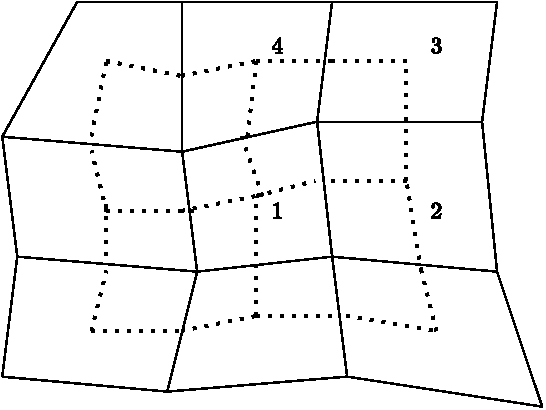
\includegraphics{dualmesh.pdf}
	
	\caption{The solid lines are the control volumes, the dashed lines are the dual mesh connecting the cell centers, going trough the midpoints of each edge.}
	\label{fig:dualmesh}
\end{figure}
For each gridpoint, that means where four control volumes intersect, we consider an interaction region. This is the polygon drawn by the dualmesh around the gridpoint.
\begin{figure}[H]
	\centering
	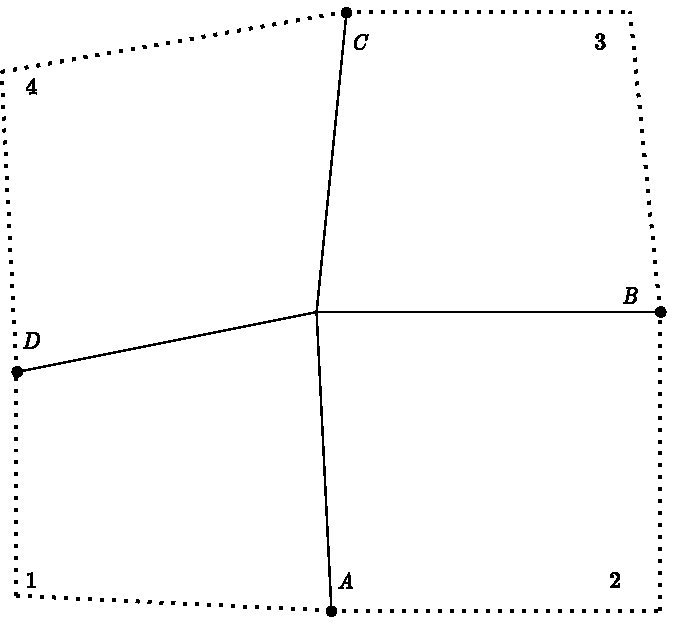
\includegraphics[width=0.6\textwidth]{Interaction region.pdf}
	\caption{The interaction region corresponding to cells $1,2,3,4$.}
	\label{fig:interactionregion}
\end{figure}
In each interaction region there are four half edges, and the flux trough each of the half edges are determined by a linear combination of the four cell center potential values. 
\begin{equation*}
	f_i = \int_{\partial \Omega_i}\hat{\pmb{n}_i}^T \pmb{K} \nabla u ds = \sum_{j=1}^4 t^j u^j \ \ i,j \in \left \{ 1,2,3,4 \right \}
\end{equation*}
Where subscript $i$ denotes the half edges of the interaction region and $j$ denotes cell center potential values.
\par
We assume for now that the potential is linear in each of the four subcells in the interaction region, figure  \ref{fig:interactionregion}. This gives $4\cdot 3 = 12$ degrees of freedom. The linear potential must ofcourse equal the cellcenter values of the potential in the cellcenters, this removes four degrees of freedom. We also require flux continuity on the four half edges in the interaction region, this removes an aditional four degrees of freedom. The last four degrees of fredom are spent on potential continuity of the midpoints of the edges. 
\par
By theese assumptions of flux and potential continuity we can calculate the transmissibility coefficients. This involves equations for flux and potential derived with properties from the mesh, see \cite{Aavatsmark2002} for the details. What we end up with is a four by four transmissibility matrix for each interaction region. Finally we assemble the system of equations \eqref{eq:fvm system} with the transmissibility coefficients. Note that we write the flux over the $j$th edge of cell $i$, $\tilde{f}_{i,j}$ as the flux over the two half edges.
\begin{equation*}
	\begin{aligned}
		\sum_{j=1}^4 (\tilde{f}_{i,j}^1 + \tilde{f}_{i,j}^2) &= |\Omega_i|F(x_i) \\
		\sum_{j=1}^4 (\sum_{k=1}^4 t^{k,1}_{i,j}u^k + \sum_{k=1}^4 t^{k,2}_{i,j}u^k)&= |\Omega_i|F(x_i)\\
	\end{aligned}
\end{equation*}
Next, we see that the interaction regions of the two half edges sharing same edge overlaps, so we get a six point flux stencil.
\begin{equation*}
	\sum_{j=1}^4 \sum_{k=1}^6 \overline{t}^{k}_{i,j}u^k = |\Omega_i|F(x_i)
\end{equation*}
We can simplify this further and see that we get a nine point stencil.
\begin{equation*}
	\sum_{k=1}^9 \hat{t}^{k}_{i,j}u^k = |\Omega_i|F(x_i)
\end{equation*}
\section*{L-method}
\addcontentsline{toc}{section}{L-method}
As the O-method, the L-method is also a multipoint flux approximation method. It was introduced in \cite{https://doi.org/10.1002/num.20320}. This method is similar to the O-method in that it goes trough the half edges and uses information from the same interaction regions. But instead of using four points for the flux across each half edge, we use three, with two half edges between them. \par
As in the O-method, we assume linear potential in each cell, this gives us $3\cdot 3 = 9$ degrees of freedom. Three are eliminated because we respect the cellcenter value of the potential, this leaves six degrees of freedom. We use two, one at each edge, for flux continuity. The last four are used for potential continuity at the two edges. 
\par
We have two choices of flux stencil for each half edge \ref{fig:two choices}. We compute the transmissibility coefficients for both, then we choose the one "best" aligned with the flow. Let $t_1^i$ be the $i$th transmissibility coefficient of $T_1$, then
\begin{equation}\label{eq:L-criterion}
	\begin{aligned}
		&\text{if} \ |t^1_1| < |t^2_2| \\
		&\text{choose} \ T_1 \ \text{else} \\
		&\text{choose} \ T_2
	\end{aligned}
\end{equation}
\begin{figure}[H]
	\centering
	\begin{subfigure}[b]{0.4\textwidth}
		\centering
		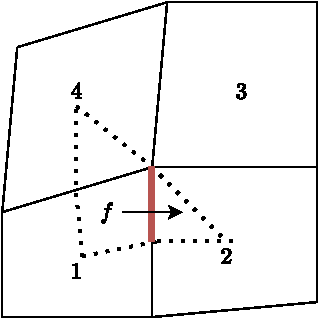
\includegraphics[width=\textwidth]{left choice.pdf}
		\caption{$T_1$}
	\end{subfigure}
	\hfill
	\begin{subfigure}[b]{0.4\textwidth}
		\centering
		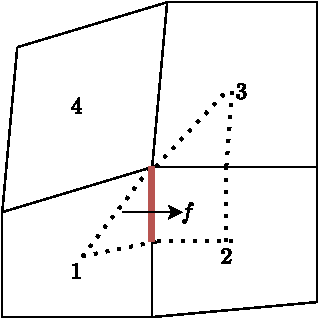
\includegraphics[width=\textwidth]{right choice.pdf}
		\caption{$T_2$}
		\label{fig:three sin x}
	\end{subfigure}
	\caption{The two choices of which cellcenters to use for computing the flux over the halfedge in red.}
	\label{fig:two choices}
\end{figure}
A cheap intuition behind \eqref{eq:L-criterion} is that if $|t_1^1|<|t_2^2|$, it is more likely that $sgn(t_1^1) = sgn(t_1^4)$ and if not, $sgn(t_2^2) = sgn(t_2^3)$ is more likely. This increases the chances that we get the same sign of $t^i$ on the same side of the half edge which is more stable. \todo{explain some more} See \cite{https://doi.org/10.1002/fld.1926} for a more detailed geometric intuition in the case of homegenous permability tensor. In figure \ref{fig:L-triangles} we see the criterion in practice for a homogenous medium. In figure \ref{fig:paralellogram-L} all L-triangles are used by two half-edges, and they are chosen in the same way troughout the domain. In figure \ref{fig:complicated-L} there are some triangles that overlap, this is due to the fact that some L-triangles are used by only one half edge.
\begin{figure}[H]
	\centering
	\begin{subfigure}[b]{0.8\textwidth}
		\centering
		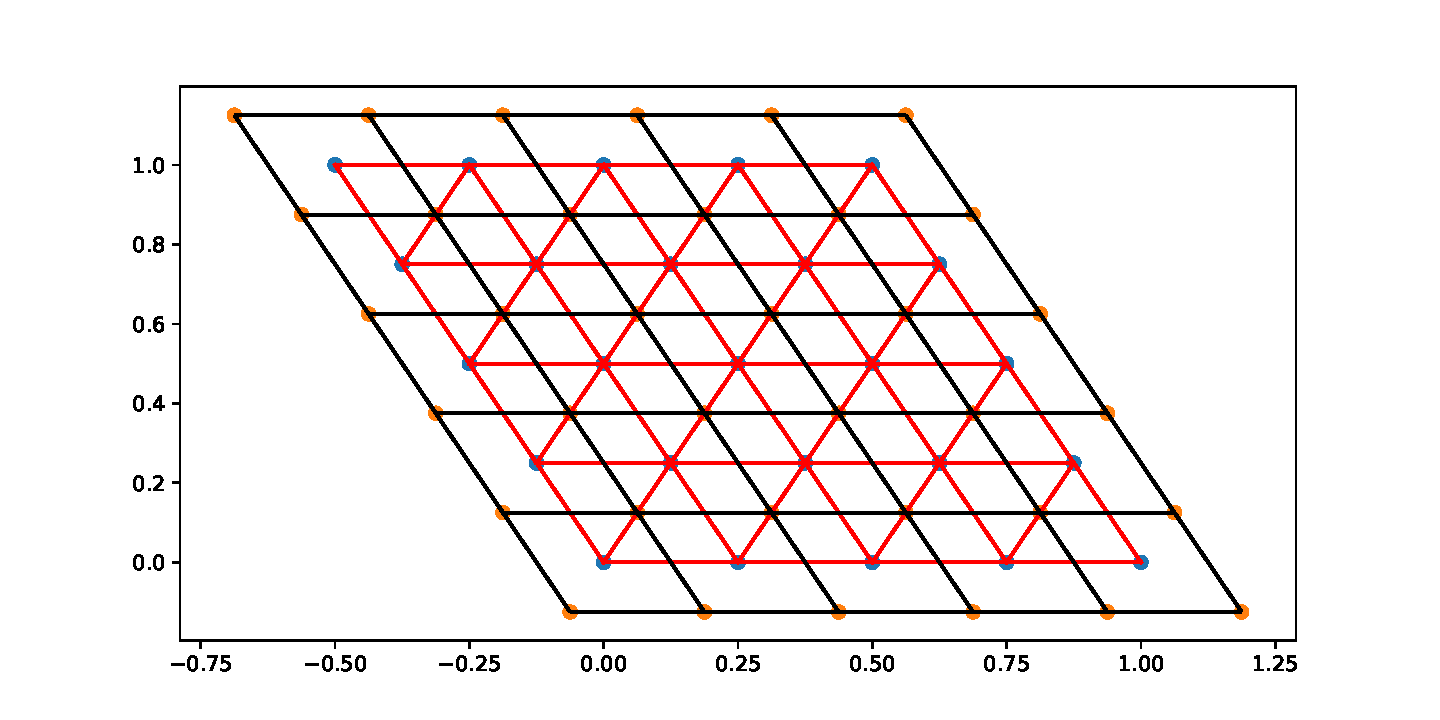
\includegraphics[width=\textwidth]{L-triangles_paralellogram.pdf}
		\caption{Paralellogram grid, all triangles are chose similarily.}
		\label{fig:paralellogram-L}
	\end{subfigure}
	\hfill
	\begin{subfigure}[b]{0.8\textwidth}
		\centering
		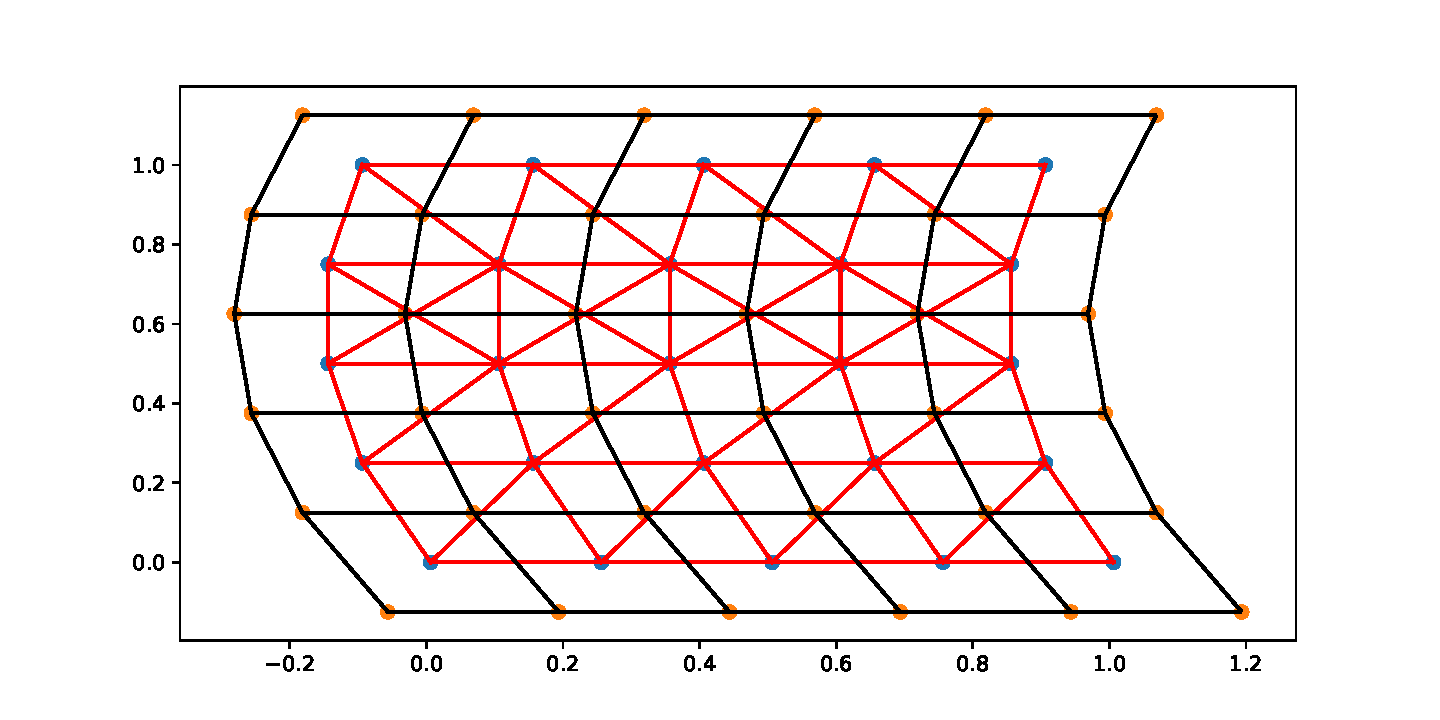
\includegraphics[width=\textwidth]{L-triangles_complex.pdf}
		\caption{Complicated grid, note that some of the L-triangles overlap.}
		\label{fig:complicated-L}
	\end{subfigure}
	\caption{Examples of L-triangles(in red) in a domain with homogenous permability tensor.}
	\label{fig:L-triangles}
\end{figure}
This observation can be stated as a theorem:
\begin{theorem}[Cao, Y., Helmig, R. and Wohlmuth, B.I. (2009),\cite{https://doi.org/10.1002/num.20525}]
	\label{th:L_triangulation}
	For homogeneous media and uniform parallelogram grids, the MPFA L-method
	has a seven-point cell stencil for the discretization of each interior cell, ie. the discretization of each cell is a seven point stencil including the center cell and the six closest potential cells, as shown in \ref{fig:paralellogram-L}.
\end{theorem}
As with the O-method, we end up with a system assembled from the fluxes over the half edges.
\begin{equation}
	\begin{aligned}
		\sum_{j=1}^4 (\tilde{f}_{i,j}^1 + \tilde{f}_{i,j}^2) &= |\Omega_i|F(x_i) \\
		\sum_{j=1}^4 (\sum_{k=1}^3 t^{k,1}_{i,j}u^k + \sum_{k=1}^3 t^{k,2}_{i,j}u^k)&= |\Omega_i|F(x_i)\\
	\end{aligned}
\end{equation}
But the flux stencil across each edge is possibly smaller, often just four points as would be the case in figure \ref{fig:paralellogram-L}. 
\par 
For homogenous media the L-method becomes easier to reason about. We finish this chapter with a useful theorem which we will use later:

	\begin{lemma}[Cao, Y., Helmig, R. and Wohlmuth, B.I. (2009),\cite{https://doi.org/10.1002/fld.1926}] \label{lemma:L_potential}
		Assume that the permability $\pmb{K}$ is homogenous on $\Omega$, then the flux trough each half edge $e$, computed by the L-method, can be written as
		\begin{equation}
			f_e = -\pmb{K} \nabla p \cdot \pmb{n}_e
		\end{equation}
		Where $\pmb{n}_e$ is the scaled normal vector to the half edge $e$, having the same length as $e$. $p$ is a linear scalar field uniquely given by the potential values at the three cellcenters chosen by the L-method.
	\end{lemma}
\end{document}